\documentclass{article}
\usepackage{graphicx} % Required for inserting images
\usepackage{pgf}
\usepackage{lmodern}
\usepackage{import}
\usepackage{booktabs}
\usepackage{tabu}
\usepackage{float}
\usepackage[hidelinks]{hyperref}
\usepackage{amsmath}
\usepackage{amsfonts}
\usepackage[margin=1in]{geometry}
\usepackage{pythonhighlight}
\usepackage[toc]{appendix}
\usepackage{placeins}

\setlength{\parskip}{1em}
\setlength{\parindent}{0em}

\begin{document}
\begin{titlepage}
    \begin{center}
        \vspace*{7cm}

        \Huge
        \textbf{Magnetic Hysteresis}

        \vspace{0.5cm}
        \LARGE
        PHYS2114 - Electromagnetism

        \vspace{1.5cm}

        \textbf{Toby Nguyen - z5416116}
    \end{center}
\end{titlepage}

\tableofcontents

\newpage

\section{Introduction}
Magnetic Hysteresis is a phenomenon arising from the make up of ferromagnets. 
Ferromagnetism involves the magnetic dipoles associated with the spins of 
unpaired electrons like in the case of paramagnetism. However, due to quantum
mechanical effects such as the Pauli exclusion principle which restricts the
occupancy of electrons' spin states in atomic orbitals, the magnetic dipoles 
in ferromagnets tend to 'like' to point in the same direction as its neighbours,
making it very distinct from paramagnetism.

Alignment of these dipoles occurs in relatively small patches, called domains.
The domains contain billions of magnetic dipoles all aligned in the same direction
with each other. Each domain is randomly orientated but can be changed by the 
influence of external magnetic fields. When an external magnetic field is deployed
over a ferromagnet, the torque $N = m \times B$ will align the dipoles parallel to
the field however aforementioned, these dipoles will resist in order to be aligned
with their neighbours. On the boundaries, there are competing neighbours and so the
torque will be most effective here, aligning the dipoles that are closest in parallel
to the field.

Once the domain wins some converts from its neighbouring domains, the boundary line 
is pushed and the domain is expanded and in consequence, the other domains in the 
ferromagnet will begin to shrink. When one domain expands enough and takes over 
entirely, the ferromagnetic material is said to be saturated. It should be noted that
the magnetic field strength will have diminishing effect on the material as once more
and more domains are converted, the difficulty or required magnetic field strength to
convert the remaining domains increase up to a saturation point.

This process, however, is not reversible. Once the magnetic field is turned off, not 
all the domains will return to their original randomly orientated alignments. Some will
but there is enough that remain aligned with the now gone magnetic field to produce a
permanent magnet. Running a magnetic field in the opposite direction of the first one 
will re-orientate some of the dipoles to remove this permanent magnet, i.e demagnetise.
Some materials will withstand this field more than others, with the property denoted as
magnetic coercivity. Magnetically hard materials, which tend to be used as permanent 
magnets have high coercivity, retaining their permanent magnet status despite the existence
of external magnetic fields whilst magnetically soft materials have low coercivity and are
such more easily demagnetised and magnetised.

This entire process is visualised in Figure \ref{fig:loop} below.

\begin{figure}[H]
    \centering
    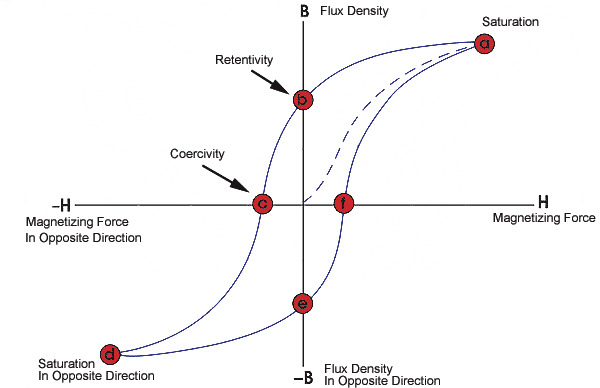
\includegraphics[width=0.8\textwidth]{loop.jpeg}
    \caption{Hysteresis loop}
    \label{fig:loop}
\end{figure}

We can see that points a and d represent the saturation points, where the one domain takes
over the material completely only under an external magnetising force. Once H goes to zero, 
i.e the external field is turned off, the material will be at points b or e, retaining some 
magnetic field. Turning on a magnetic field in the opposite direction will bring the material
to points c and f, a state of complete demagnetisation as all the domains cancel out each other
before repeating the process once the field is turned on to be stronger. Note the dotted line,
the virgin curve, will represents the process in which the material is first put in a magnetic
field. At the origin, the material's domains are randomly orientated and so once magnetised, it
cannot go back into that state again without undergoing a phase transition. This is why 
ferromagnets have magnetic history, and its magnetisation is dependent on its state in the 
hysteresis loop.

The most common way to demagnetise a permanent magnet is to place it in a region of zero magnetic
field and then heat it up above the Curie point. This will turn the ferromagnet into a paramagnet 
destroying the previous alignments of the domains. There are other ways such as just simply dropping
the magnet onto a hard surface or placing it between the poles of an electromagnet and then magnetise
it back and forth whilst reducing the current to reduce the field slightly but none of these methods
will return the magnet to the exact state in which it was before.

\section{Aim}
The aim of this experiment is to validate the model of the hysteresis loop shown in Figure \ref{fig:loop}
and thus the interpretation of the microscopic interactions of dipoles explored in the previous section.
By studying the interaction of traditional ferromagnetic materials with an applied magnetic field, we can
gain some insights into the how the microscopic physical model of magnetism relates to macroscopic fields.

\section{Method}
\subsection{Theory}
The auxiliary field is denoted with $H$ and it represents the magnetic field produced by free current,
\begin{equation}
    H = \frac{1}{\mu_0}B-M
\end{equation}

where B is total magnetic field strength and M is the magnetic dipole moment per unit volume in a region.

In linear media, the magnetisation of materials is proportional to the field $H$, not $B$, so
\begin{equation}
    M = \chi_m H
\end{equation}

where $\chi_m$ is the magnetic susceptibility of the material. 

Thus,

\begin{equation}
    B=\mu_0(H+M)=\mu_0(1+\chi_m)H.
\end{equation}

So,

\begin{equation}
    B = \mu H.
\end{equation}

\subsection{Experimental Setup}
To explore the relationship between $H$ and $B$ for a ferromagnet, the following circuit is set up in
Figure \ref{fig:circuit} below.

\begin{figure}[H]
    \centering
    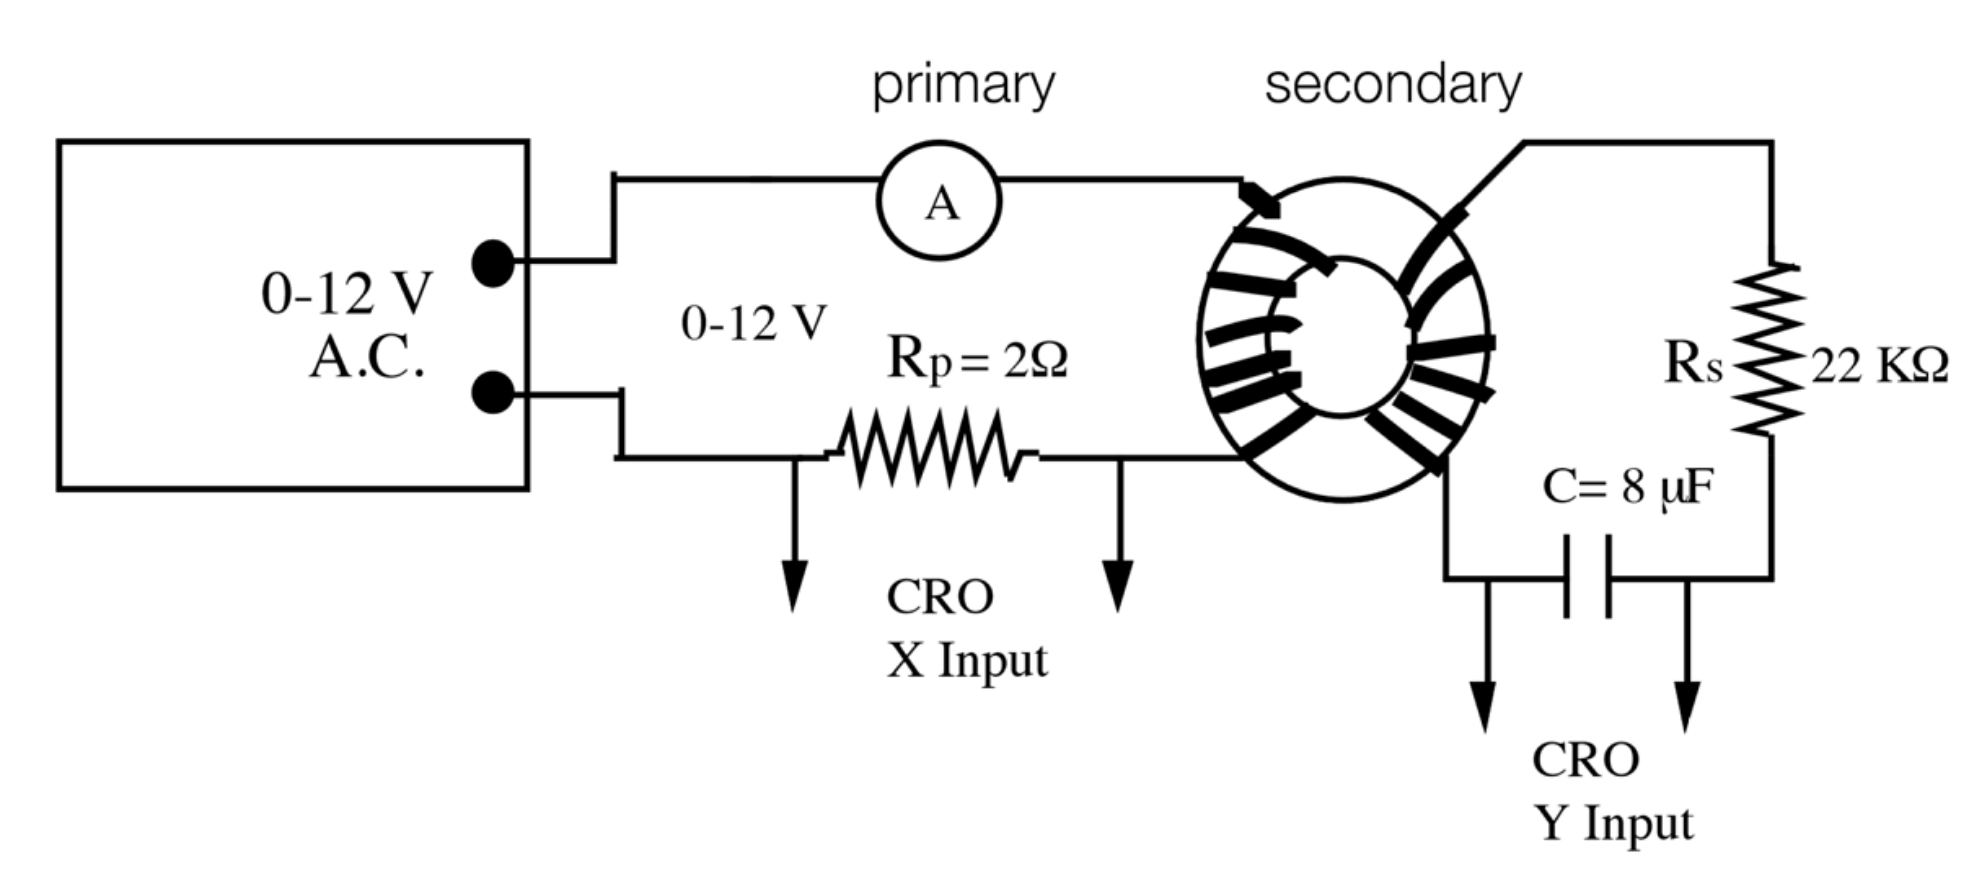
\includegraphics[width=0.8\textwidth]{circuit.png}
    \caption{Circuit diagram of the setup}
    \label{fig:circuit}
\end{figure}

There is a primary circuit measuring $H$ and a secondary circuit measuring $B$ which are both connected
to the same oscilloscope with two different channels. In the case of a toroidal transformer, the magnetising
$H$ field is produced by the current $I$ in the primary coil,

\begin{equation}
    H = \frac{n_pI}{2\pi r}.
\end{equation}

The varying $B$ field in the core of the toroid induces a voltage in the secondary coil,

\begin{equation}
    V_s = n_sA\frac{dB}{dt}.
\end{equation}

Rearranging for $B$ gives,

\begin{equation}
    B = \frac{1}{n_s A} \int V_s dt.
\end{equation}

To obtain the signal proportional to B, we must integrate the secondary voltage.

For a varying voltage $V_{in}$ applied to a resistor and capacitor in series, the
potential difference at the capacitor is

\begin{equation}
    V_C = \frac{Q}{C} = \frac{1}{C}\int I dt
\end{equation}

where $I$ is the current flowing through the resistor and into the capacitor.

If $V_C \ll V_{in}$ then the voltage across the resistor is almost equal to $V_{in}$ and so,

\begin{equation}
    I = \frac{V_{in}}{R}.
\end{equation}

Thus,

\begin{equation}
    V_C = \frac{1}{RC} \int V_{in} dt.
\end{equation}

In the case above, the input voltage $V_{in}$ is $V_s$ and the voltage across the capacitor can
be measured by the oscilloscope so we have,

\begin{equation}
    B = \frac{R_s C}{n_s A}V_Y
\end{equation}

and 

\begin{equation}
    H = \frac{n_p}{2\pi r R_p}V_X
\end{equation}

where $V_X$ and $V_Y$ are the voltage readings across the resistor and capacitor respectively 
displayed in Figure \ref{fig:circuit}.

\subsection{Energy Dissipation}
To find the energy dissipated by the toroid in one cycle, we will use the following equation,

\begin{equation}
    E = \frac{n_pR_sC}{2\pi n_s R_p r A}S
\end{equation}

where S is the area of the hysteresis loop. To obtain S we will be using two methods. Numerical
integration involves the use of scipy.integrate package, where we can use Trapezoidal and Simpson
rule to obtain two values of the area of the curves. The second method is to cut and weigh the 
graph. The top left hysteresis curve in Figure \ref{fig:loops} is cut out and weighed to find the
area S using the formula,

\begin{equation}
    S = (2)(0.1)\frac{m_{outer}+m_{inner}}{2m_{total}}
\end{equation}

where the $2$ and $0.1$ are the adjustment factors for the scaling of the graph.

\subsection{Remanent Magnetisation}
The remanent magnetisation of a magnet will occur at point b in the hysteresis loop in Figure \ref{fig:loop}.
To find the relationship between $B_{re}$ and $H$, a plot of the remanent magnetisation against $H$ will
be produced. The limiting value of $B_{re}$ can be calculated as $H\rightarrow \infty$.

\subsection{Systematic Uncertainties} \label{sec:sigma}
The main drivers of systematic uncertainty would be the input voltage from the VARIAC and the oscilloscope used
to measure $V_X$ and $V_Y$. Upon looking at their manuals, no uncertainty values were given so we're going to 
assume the combined Uncertainties from these two instruments will be 5\% which will be the total systematic uncertainty.

\section{Results}

\begin{figure} [H]
    \subsection{Hysteresis Loop}
    \centering
    \scalebox{0.75}{\input{loop2.pgf}}
    \label{fig:loopexp}
    \caption{Hysteresis Loop found experimentally for I = 1.6A.}
\end{figure}

\FloatBarrier

\begin{figure}[p] \label{fig:loops}
    \subsection{Numerical Integration curves}
        \centering
        \scalebox{0.52}{\input{loop1.pgf}}
        \hspace{0.5cm}
        \scalebox{0.52}{\input{loop3.pgf}}
      
        \vspace{0.5cm}
      
        \scalebox{0.52}{\input{loop4.pgf}}
        \hspace{0.5cm}
        \scalebox{0.52}{\input{loop5.pgf}}
      
        \vspace{0.5cm}
      
        \scalebox{0.52}{\input{loop6.pgf}}
        \hspace{0.5cm}
        \scalebox{0.52}{\input{loop7.pgf}}
      
        \caption{Top left curve is the sum of the 5 loops found experimentally.}
    \end{figure}

\FloatBarrier

\begin{figure} [H]
    \subsection{Plot of Remanent Magnetisation}
    \centering
    \scalebox{0.75}{\input{curve1.pgf}}
    \label{fig:curveexp}
    \caption{Logistic curve fitted onto the graph.}
\end{figure}

\section{Analysis}
\subsection{Energy Dissipation}
\subsubsection{Numerical Integration}
For the numerical integration using the trapezoidal rule the area value obtained over 1 cycle is 
the average of the absolute value of the areas found in the 5 cycles above. So,

\begin{equation}
    \begin{split}
    S_{avg} &= \frac{0.0098 + 0.0162 + 0.0051 + 0.0219 + 0.0198}{5} \\
    S_{avg} &= 0.01456 V^2.
    \end{split}
\end{equation}

The uncertainty of this value is found by taking the difference between the max value and min value
and dividing by two,

\begin{equation}
    \begin{split}
    \sigma &= \frac{max - min}{2} \\    
    &= \frac{0.0219 - 0.0051}{2} \\
    &= 0.0084.
    \end{split}
\end{equation}

Combining the statistical uncertainty with the systematic uncertainty found in Section \ref{sec:sigma} 
will give, 

\begin{equation}
    \begin{split}
    sigma_{total} &= \sqrt{(\frac{0.0084}{0.01456})^2+0.05^2} \\
    &= 57.9\%.    
    \end{split}
\end{equation}

So the area value obtained by the trapezoidal rule is given as $0.01328 \: \pm \: 0.0084 V^2$, 
representing a 58\% uncertainty value.

Similarly, for Simpson's rule, the value obtained is $0.06012 \: \pm \: 0.041 V^2$, representing 
a 69\% uncertainty value.

\subsubsection{Cut and Weigh}
The total mass of the paper was 3.00g whilst the mass of the outer curve was 0.47g and the inner 
curve was 0.34g. The grid was made up of 64 2V by 0.2V squares, making the area of the curve,
\begin{equation}
    \begin{split}
        S &= (0.2)(2)\frac{0.47+0.34}{2*3} \\
        &= 0.054 \text{V\textsuperscript{2}}.
    \end{split}
\end{equation}

The uncertainty of this measurement is driven mainly by the aforementioned systematic uncertainties
but also the uncertainty of the cutting, adding another 1\% error to the measurement.

Thus,

\begin{equation}
    S = 0.054 \: \pm \: 0.0027 \text{V\textsuperscript{2}}.
\end{equation}

\subsubsection{Energy Dissipation}
From the value of S, the energy dissipated per volume per cycle is given by,

\begin{equation}
    E = \frac{n_p R_s C}{2\pi r R_pA}S.
\end{equation}

We find the energy dissipated per volume per cycle of the S value found using the trapezoidal rule
to be,

\begin{equation}
    \begin{split}
        E &= \frac{(584)(21892)(9.9741\times 10^{-6})}{(2\pi)(0.05)(1.9703)(0.00006)}(0.01456) \\
        &= (4441.8)(0.01456) \\
        &= 64.67 \: \text{Jm\textsuperscript{-3}/cycle}.
    \end{split}
\end{equation}

Using the value of S from the Simpson's rule we find that,

\begin{equation}
    \begin{split}
        E &= (4441.8)(0.06012) \\
        &= 267.04 \: \text{Jm\textsuperscript{-3}/cycle.}
    \end{split}
\end{equation}

The value of S found from the cut and weigh came out to be 0.054, using this to find E,

\begin{equation}
    E = 239.86 \: \text{Jm\textsuperscript{-3}/cycle}.
\end{equation}

The corresponding uncertainties are then, 

\begin{equation}
    \begin{split}
    E_{trapz} &= 64.67 \: \pm \: 37.5\: \text{Jm\textsuperscript{-3}/cycle}, \\
    E_{simps} &= 267.04 \: \pm \: 184.26 \: \text{Jm\textsuperscript{-3}/cycle}. \\  
    E_{cw} &= 239.86 \: \pm \: 12 \: \text{Jm\textsuperscript{-3}/cycle}
    \end{split}
\end{equation}

The volume of the toroid is given by the formula,
\begin{equation}
    V = (\pi r^2) (2\pi R).
\end{equation}

Given that $A=\pi r^2 = h \times w = (0.03)(0.0002) = 0.00006 \text{m\textsuperscript{2}}$,
the volume is then,

\begin{equation}
    \begin{split}
        V &= (0.00006)(2\pi)(0.05) \\
        &= 1.88 \times 10^{-5} \text{m\textsuperscript{3}}.
    \end{split}
\end{equation}

Thus the total power loss with a 50Hz frequency as calculated for each $E$ will be, 
$P_{trapz} = 0.061 \: W$, $P_{simps} = 0.251 \: W$ and $P_{cw} = 0.225 \: W$.

\subsection{Remanent Magnetisation}
The logistic curve fit onto Figure \ref{fig:curveexp} is given by the equation,

\begin{equation}
    f(x) = \frac{L}{1+e^{-k(x-x_0)}}.
\end{equation}

The fitted parameters are then, $L=0.023$, $k =0.081$ and $x_0 = 294.2307$.

As $x \rightarrow \infty$, we find that $f(x) \rightarrow L$ so the limiting value of the remanent
magnetisation is then 0.023T. The minimum value of the applied field intensity required to produce 
the strongest magnet from the core material of the toroid by momentary immersion in this field $H_m$
can be found by taking the regression line and solving for $x$ when $f(x)$ is 95\% of the limiting 
value of $B_{re}$. It is found by,

\begin{equation}
    f(x) > 0.95*0.023=0.02185.
\end{equation}

This occurs for $x > 657.74$ or a value of $H_m$ greater than 658 A/m.

\section{Discussion}
We find that the results for energy dissipation come with high uncertainty with
the trapezoidal rule producing a value of $0.01328 \: \pm \: 58\%$ and the Simpson's 
rule producing an area value of $0.06012 \: \pm \: 69\%$. To reduce uncertainties 
in future experiments we can take more cycles of the hysteresis loops and use a 
standard deviation measure for our uncertainty. We can also use a less volatile VARIAC
to reduce randomness in the voltage input and thus the current. The integration method
itself is less effective for less smooth curves so obtaining more data points to smoothen
out the curve would improve the accuracy of the reading.

The cut and weigh method provided a much lower uncertainty value of 5\%. Out of the three methods,
this would be the most accurate. We notice that the area value found by using cut and weigh
method being $S = 0.054 \: \pm \: 0.0027\text{V\textsuperscript{2}}$, agrees with the Simpson's rule
integration method, mainly due to the high uncertainty of the numerical integration. Taking the cut and 
weigh's value of area, turning it into energy dissipated per volume per cycle gives $E = 239.86 \: \pm
\: 12 \text{Jm\textsuperscript{-3}/cycle}$. Finally the power loss is calculated to be $P = 0.225 \: \pm
\: 0.01 \: W$. The maximum power loss of the circuit is given as $P = VI$ where V = 12V input voltage and I = 1.6A,
combining to be 19.2 W.

In the remanent magnetisation experiment, the residuals of each data point is quite high
indicating higher variance in the data collected. To obtain a more accurate measure of 
error, more trials should have been taken to obtain a statistical uncertainty as well as 
reducing residuals as the mean for each data point could have been used. To reduce systematic 
uncertainty we can use less volatile VARIAC and more accurate oscilloscope.

\section{Conclusion}
Although the experiment can be majorly improved with greater uncertainty analysis, the overall aim was 
tested and the relationship between the auxiliary field, H and its effect on the 
magnetic field strength of the ferromagnet was seen and verified, indicating validity in the 
interaction between the microscopic model of magnetism and how it relates to macroscopic fields.

\appendix
\section{Prework}
\begin{figure}[H]
    \centering
    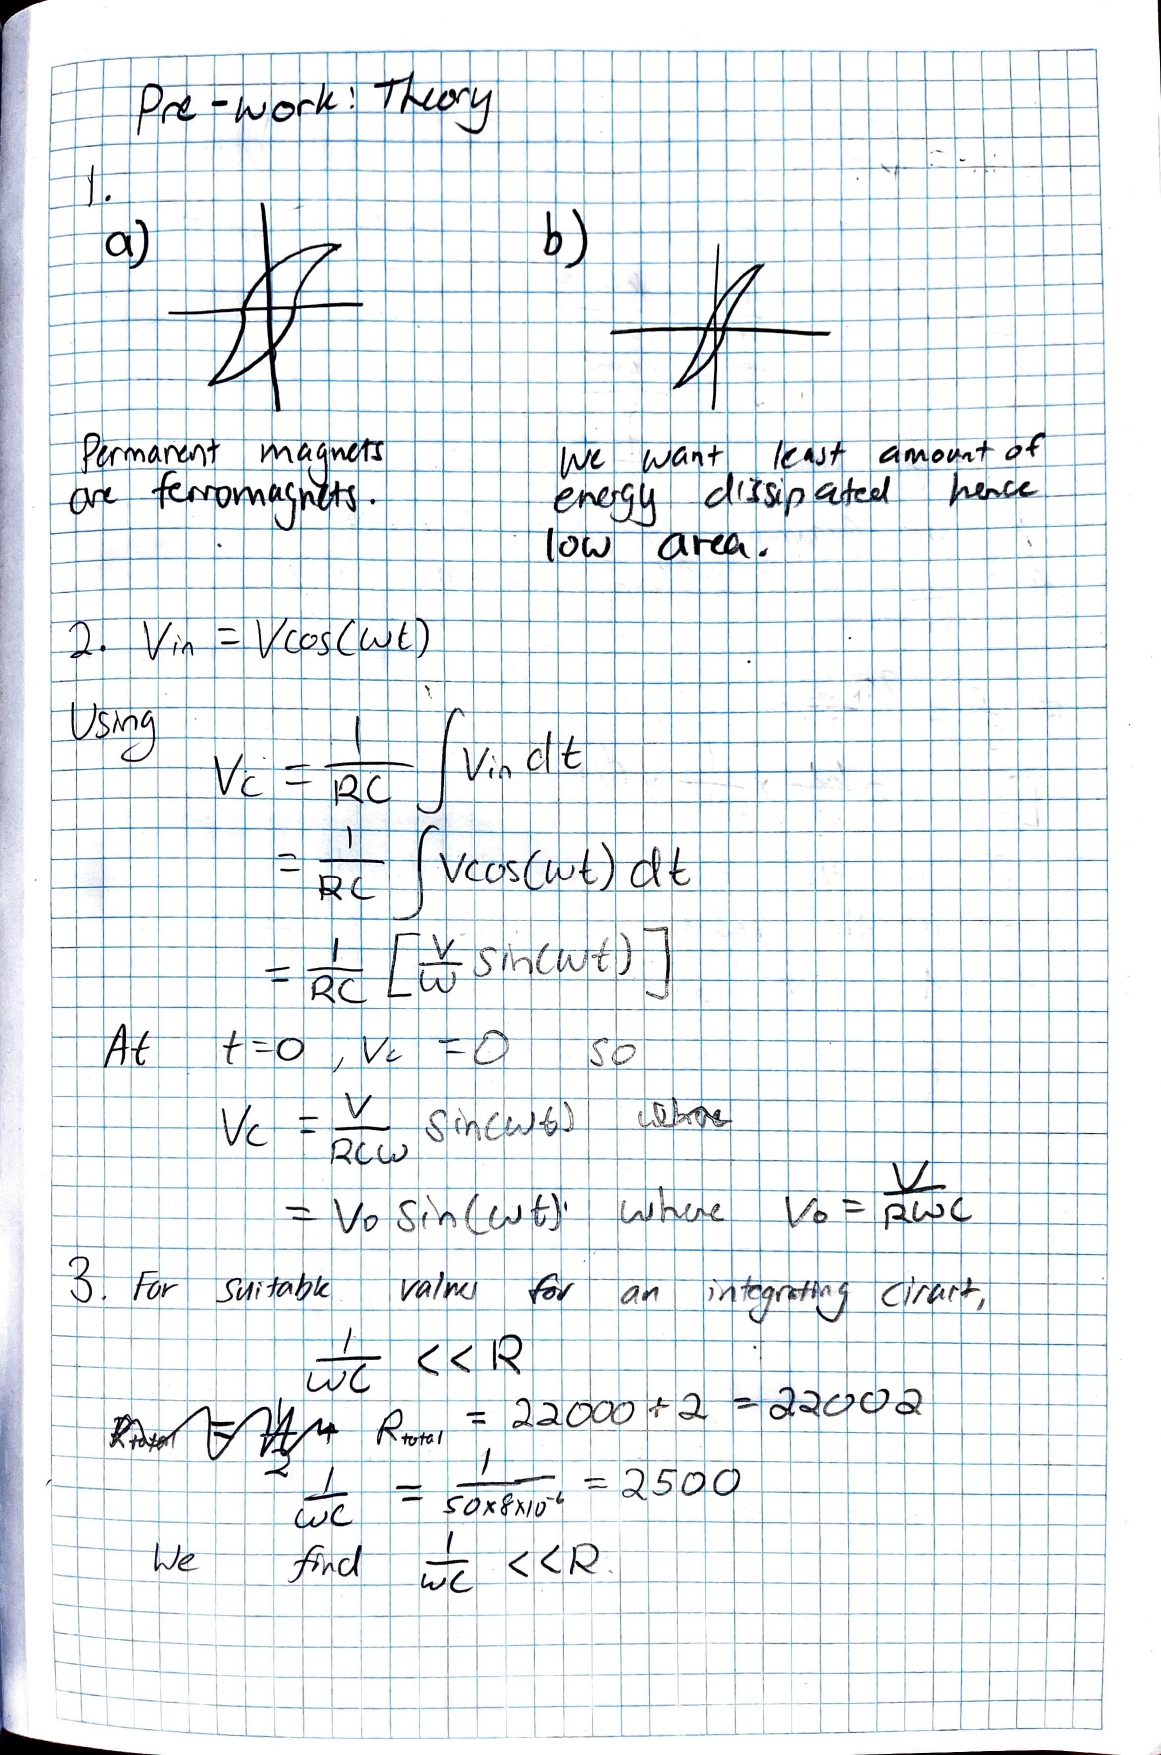
\includegraphics[width=0.8\textwidth]{prework1.jpg}
    \caption{Prework Theory.}
\end{figure}
\begin{figure}[H]
    \centering
    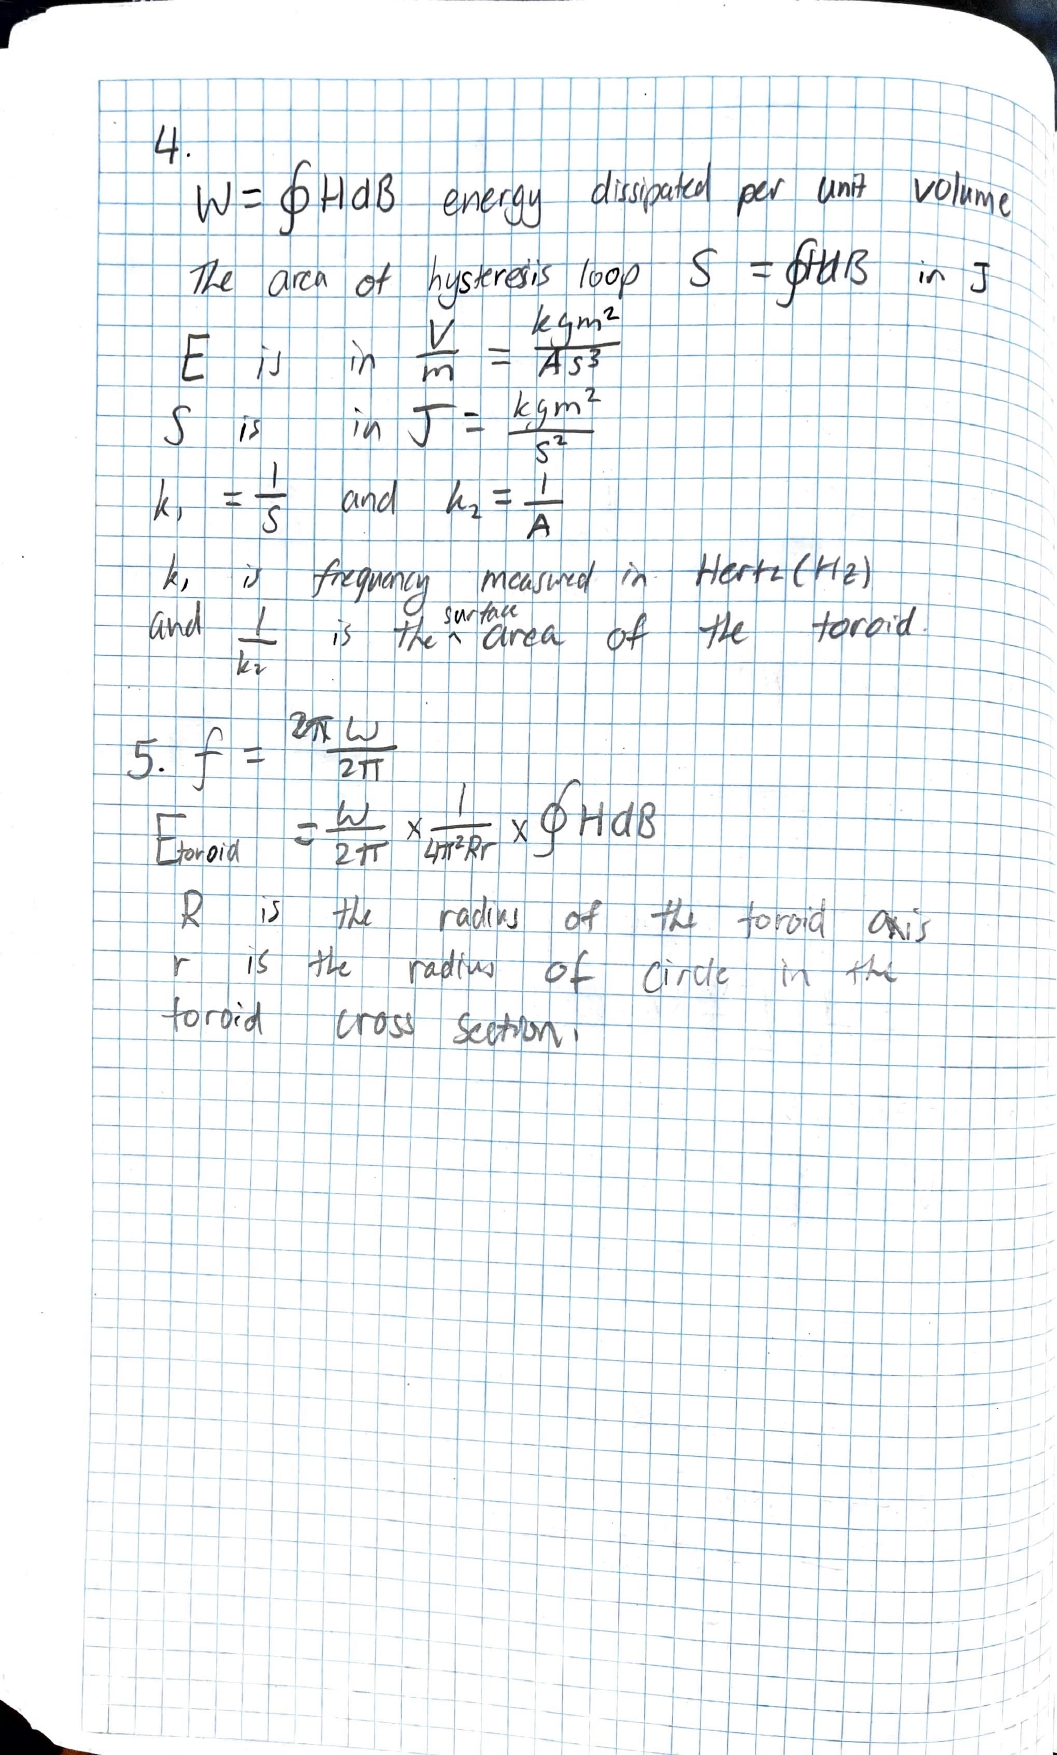
\includegraphics[width=0.8\textwidth]{prework2.jpg}
    \caption{Prework Theory.}
\end{figure}

\subsection{Corrections}
For Question 1a, permanent magnets have thicker hysteresis loops as to better retain their 
remanent magnetisation.

For Question 3, the resistance of the integrating circuit should just be 22000 Ohms, although
this will not affect the final conclusion.

For Question 4, $k_1 = \frac{n_p}{2\pi r R_p}$ and $k_2 = \frac{R_s C}{n_s A}$. Energy, $E$,
is measured in Joules (J). The area of the hysteresis curve for $V_X$ and 
$V_Y$ will be in $V^2$. $k_2$ contains Farads which are equivalent to $\frac{J}{V^2}$. The 
remaining $A$ in $k_2$ and $2\pi r$ in $k_1$ will represent the volume of the toroid.

\section{Lab Notes}
\begin{figure}[H]
    \centering
    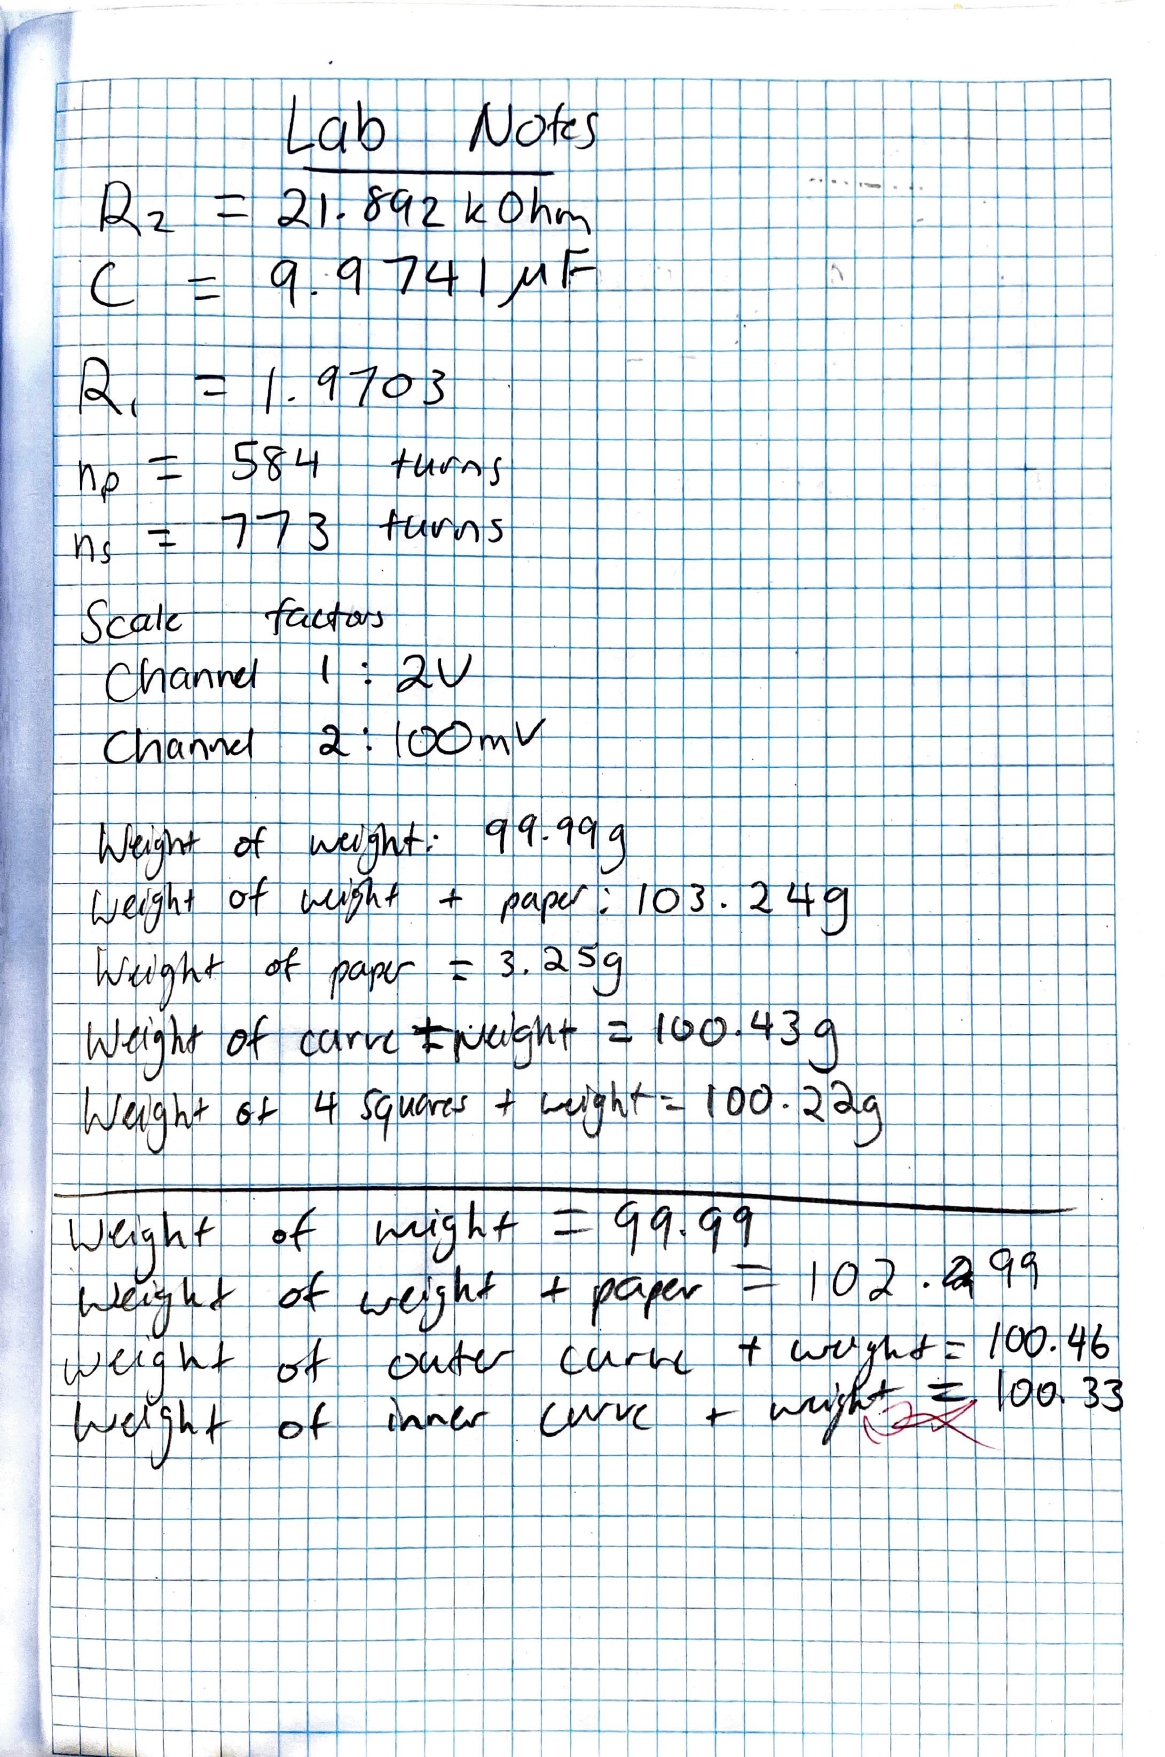
\includegraphics[width=0.8\textwidth]{labbook.jpg}
    \caption{Signed Lab book.}
\end{figure}

\begin{python}
plt.scatter(
    dfna['R_gc'],
    dfna['sig_v'],
    marker='x',
    c=dfna['[Fe/H]']
)

plt.xlim(0,30)
plt.xlabel("Galactic Radius (kpc)")
cbar = plt.colorbar()
cbar.set_label('[Fe/H]')
plt.ylabel("Dispersion velocity (km/s)")
plt.savefig("rgcsigv1.pgf", bbox_inches='tight', pad_inches=0.1)
\end{python}

\begin{python}

\end{python}
\end{document}